\newpage
\section{Die elektrische Leistung}


Die elektrische Leistung $P$ ist definiert als das Produkt der Spannung $U$ und der Stromstärke $I$. Die Einheit der Leistung ist
das Watt ($\unit{\watt}$).


\begin{greenbox}
\textbf{Elektrische Leistung $P$}
$$
    P = U * I \quad,\quad \left[ P \, \right] = \unit{\volt} * \unit{\ampere} = \unit{\watt} \quad \text{(Watt)}
$$
\end{greenbox}



\exercise{Formel herleiten}

Die Leistung $P$ ist das Verhältnis der Energie $E$ zu der Zeit $t$.
Zeige, dass das Produkt aus Spannung und Stromstärke gleich der Leistung ist.
Überprüfe anschliessend auch die Einheiten, d.h. zeige, dass Volt mal Ampere gleich Watt ist.

% Raster für die Antworten
\begin{tikzpicture}
    \draw[step=4mm,gray,very thin] (0,0) grid (14.8,-4);

    \answer{
        \draw (0.3,-0.4) node[anchor=north west,align=left,text width=13cm] {%
      		\marker%
            $$
                U * I = \frac{E}{Q} * \frac{Q}{t} = \frac{E}{t} = P
            $$

            $$
                \unit{\volt} * \unit{\ampere} = \frac{\unit{\joule}}{\unit{\coulomb}} * \frac{\unit{\coulomb}}{\unit{\second}} = \frac{\unit{\joule}}{\unit{\second}} = \unit{\watt}
            $$
        };
    }

\end{tikzpicture}



\exercise{P-I-Diagramm einer Glühbirne}

Erstelle ein Diagramm der Leistung $P$ einer Glühbirne als Funktion der Stromstärke $I$.
Verwende dazu die Formel $P = U * I$ und die Werte für die Spannung $U$ und die
Stromstärke $I$ der Glühbirne.

% Raster für die Antworten
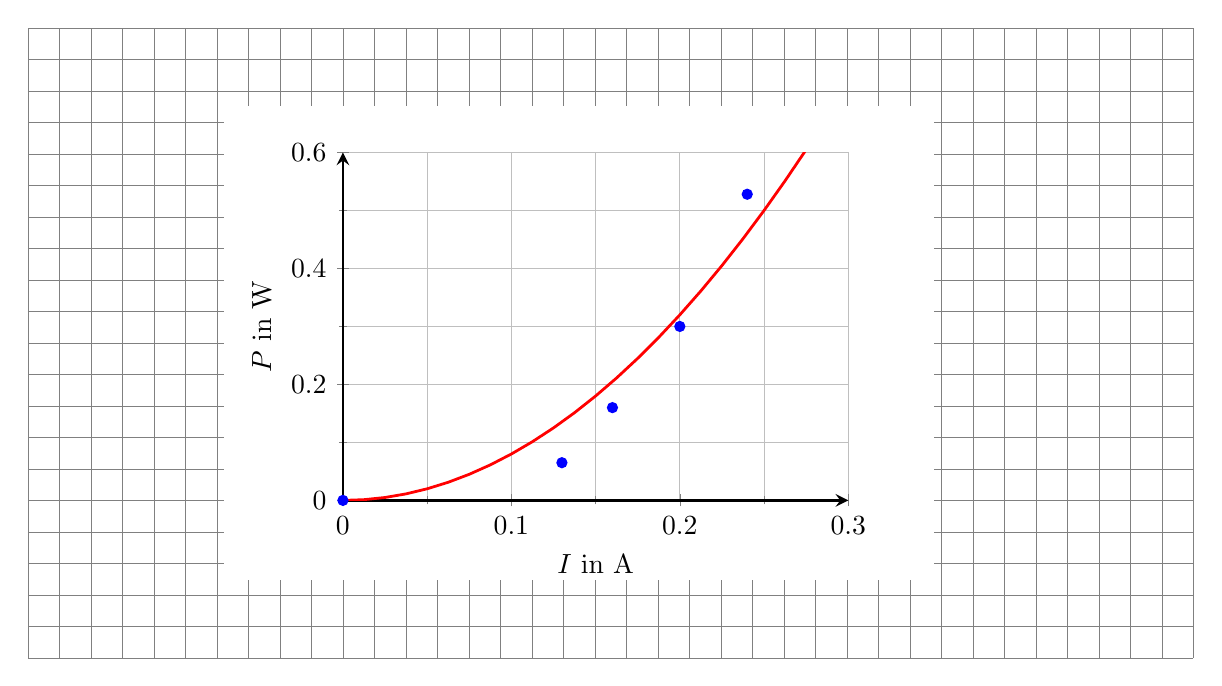
\begin{tikzpicture}
    \draw[step=4mm,gray,very thin] (0,0) grid (14.8,-8);

    \begin{scope}[shift={(4,-6)}]
        \draw[color=white,fill=white] (-1.5,-1) rectangle (7.5,5);
        \begin{axis}[
                axis background/.style={fill=white},
                axis lines=left,
                xlabel=$I$ in A,
                ylabel=$P$ in W,
                xtick={0,0.1,0.2,0.3,0.4},
                ytick={0,0.2,0.4,0.6},
                minor tick num=1,
                grid=both,
                xmin=0.0, xmax=0.3,
                ymin=0, ymax=0.6,
                line width=1pt,
                height=6cm,
                width=8cm,
                domain=0:0.3,
            ]
            \answer{
                \addplot[
                    only marks,
                    mark=*,
                    mark size=1.5,
                    color=blue,
                ] coordinates
                {
                    (0,0)
                    (0.13, 0.065)
                    (0.16,0.16)
                    (0.2,0.3)
                    (0.24,0.528)
                };

                \answer{
                    \addplot[
                        color=red,
                        domain=0:0.3,
                    ] {8*x^2};
                }
            }
        \end{axis}
    \end{scope}

\end{tikzpicture}
